\section{实验原理}

深度学习是机器学习的一个分支,它的目标是模拟人脑的神经元从而识别模式。深度学习的核心是神经网络,神经网络通过多层神经元进行连接,每一层神经元都会对输入数据进行处理,最终输出结果。深度学习的训练过程是通过大量的数据进行训练,通过不断调整神经元之间的连接权重,使得神经网络的输出结果与实际结果尽可能接近。本章节将介绍神经网络的结构、优化方法和数据增强技术。

\subsection{神经网络的结构}

神经网络中的一些常见模块包括全连接层、卷积层、池化层、激活函数等。其中,全连接层是最简单的神经网络模块,它将输入数据的每一个特征都与神经元进行连接,通过调整权重来实现特征的提取。全连接是一种线性变换操作,其中需要学习的参数有权重和偏置。具体来说,全连接操作可以表示为公式\ref{eq:fc}:

\begin{equation}
    y = Wx + b
    \label{eq:fc}
\end{equation}

其中,$x$是输入数据,$W$是权重,$b$是偏置,$y$是输出数据。全连接层结构简单,但是参数量大,容易过拟合。

卷积层是一种常用的神经网络模块,它通过卷积操作实现对输入数据的特征提取。卷积层的核心是卷积操作,后者通过滑动窗口的方式对输入数据进行处理,从而提取特征。卷积操作可以表示为公式\ref{eq:conv}:

\begin{equation}
    y_i = \sum_{i=1}^{n} x_i \cdot W_i + b
    \label{eq:conv}
\end{equation}

其中,$x_i$是输入数据的第$i$个特征,$W_i$是卷积核的第$i$个权重,$b$是偏置,$y$是输出数据。卷积操作通过共享卷积核权重和局部连接的方式,减少了参数量,提高了模型的泛化能力。同时,卷积操作模仿了人类视觉系统的工作原理,提取了输入数据的空间特征。

池化层是一种常用的神经网络模块,它通过池化操作实现对输入数据的降维处理。池化层的核心是池化操作,后者通过滑动窗口的方式对输入数据进行处理,从而降低数据的维度。池化操作可以表示为公式\ref{eq:pool}:

\begin{equation}
    y_ij = \phi_{(p,q)\in R_{ij}} x_{pq}
    \label{eq:pool}
\end{equation}

其中,$x_{pq}$是输入数据的第$(p,q)$个特征,$R_{ij}$是池化范围,$\phi$是池化操作,可以使用最大池化$\max$、平均池化$\frac{1}{|R_{ij}|}\sum$等。池化操作通过减少数据的维度,提高了模型的计算效率,同时保留了输入数据的主要特征。

激活函数是一种常用的神经网络模块,它通过非线性变换实现对输入数据的处理,使得网络拥有更强的表达能力。激活函数的常见类型包括ReLU、Sigmoid、Tanh等。这些激活函数如图\ref{fig:activation}所示。其中,ReLU是一种简单的激活函数,它将所有负数输入映射为0,保留正数输入。Sigmoid是一种常用的激活函数,它将输入映射到$(0,1)$之间,可以用于二分类问题。Tanh是一种常用的激活函数,它将输入映射到$(-1,1)$之间。此外,还有其他激活函数,如Softmax、Leaky ReLU、ELU等,这些激活函数是为了用于多分类,以及解决ReLU的失活问题而提出的。

% 通过tikz绘制激活函数图像
\begin{figure}[H]
    \centering
    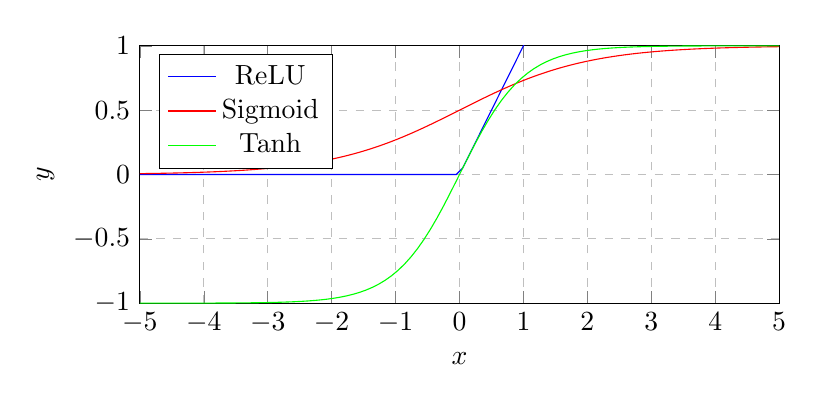
\begin{tikzpicture}
        \begin{axis}[
            width=0.8\textwidth,
            height=0.4\textwidth,
            xlabel={$x$},
            ylabel={$y$},
            xmin=-5, xmax=5,
            ymin=-1, ymax=1,
            xtick={-5, -4, -3, -2, -1, 0, 1, 2, 3, 4, 5},
            ytick={-1, -0.5, 0, 0.5, 1},
            legend pos=north west,
            grid=both,
            grid style=dashed,
        ]
        
        \addplot[blue, domain=-5:5, samples=100]{max(0, x)};
        \addlegendentry{ReLU}
        
        \addplot[red, domain=-5:5, samples=100]{1/(1+exp(-x))};
        \addlegendentry{Sigmoid}
        
        \addplot[green, domain=-5:5, samples=100]{tanh(x)};
        \addlegendentry{Tanh}
        
        \end{axis}
    \end{tikzpicture}
    \caption{激活函数图像}
    \label{fig:activation}
\end{figure}

\subsection{神经网络的优化方法}

神经网络的优化方法是指通过调整神经网络的参数,使得神经网络的输出结果与实际结果尽可能接近。神经网络最通用的优化方法是梯度下降法,它通过计算损失函数的梯度,调整参数的值,使得损失函数的值不断减小,梯度下降法可以表示为算法\ref{alg:gd}:

\begin{algorithm}[H]
    \caption{梯度下降法}
    \label{alg:gd}
    \begin{algorithmic}[1]
        \State 初始化参数$\theta$
        \While {模型未收敛}
            \State 计算损失函数$J(\theta)$和梯度$\nabla J(\theta)$
            \State 更新参数$\theta = \theta - \alpha \nabla J(\theta)$
        \EndWhile
    \end{algorithmic}
\end{algorithm}

其中,$\theta$是参数,$J(\theta)$是损失函数,$\nabla J(\theta)$是损失函数的梯度,$\alpha$是学习率。具体来说,梯度下降法具体有批量梯度下降法、随机梯度下降法、小批量梯度下降法等。这些变种的区别在于计算梯度的方式,批量梯度下降法是在整个数据集上计算梯度,随机梯度下降法是在单个样本上计算梯度,小批量梯度下降法是在一小部分样本上计算梯度。

梯度下降法是一种常用的优化方法,但是它存在一些问题,如收敛速度慢、容易陷入局部最优解等。此外,梯度下降法对学习率敏感,学习率过大容易导致震荡,学习率过小容易导致收敛缓慢。为了解决这些问题,研究者提出了一些改进的优化方法,如动量法、Adagrad、RMSprop、Adam等。这些方法通过引入动量、自适应学习率等机制,提高了优化的效率和稳定性。

动量法是一种常用的优化方法,它通过引入动量项,使得参数更新更加平滑。动量法可以表示为算法\ref{alg:momentum}:

\begin{algorithm}[H]
    \caption{动量法}
    \label{alg:momentum}
    \begin{algorithmic}[1]
        \State 初始化参数$\theta$,动量参数$\beta$
        \State 初始化动量$v = 0$
        \While {模型未收敛}
            \State 计算损失函数$J(\theta)$和梯度$\nabla J(\theta)$
            \State 更新动量$v = \beta v + (1 - \beta) \nabla J(\theta)$
            \State 更新参数$\theta = \theta - \alpha v$
        \EndWhile
    \end{algorithmic}
\end{algorithm}

其中,$\beta$是动量参数,$v$是动量,$\alpha$是学习率。动量法通过引入动量机制,动量像是现实生活中的“惯性”,使得当前参数的更新方向不仅取决于当前梯度,还取决于历史梯度,从而减少了参数更新的震荡,提高了优化的效率。

Adam是目前最常用的优化方法之一,它综合了动量法和RMSprop的优点,具有较好的优化效果。Adam可以表示为算法\ref{alg:adam}:

\begin{algorithm}[H]
    \caption{Adam}
    \label{alg:adam}
    \begin{algorithmic}[1]
        \State 初始化参数$\theta$,动量参数$\beta_1$,RMSprop参数$\beta_2$
        \State 初始化动量$v = 0$,RMSprop$s = 0$
        \While {模型未收敛}
            \State 计算损失函数$J(\theta)$和梯度$\nabla J(\theta)$
            \State 更新动量$v = \beta_1 v + (1 - \beta_1) \nabla J(\theta)$
            \State 更新RMSprop$s = \beta_2 s + (1 - \beta_2) (\nabla J(\theta))^2$
            \State 修正动量和RMSprop$\hat{v} = \frac{v}{1 - \beta_1^t},\hat{s} = \frac{s}{1 - \beta_2^t}$
            \State 更新参数$\theta = \theta - \alpha \frac{\hat{v}}{\sqrt{\hat{s}} + \epsilon}$
        \EndWhile
    \end{algorithmic}
\end{algorithm}

其中,$\beta_1$是动量参数,$\beta_2$是RMSprop参数,$v$是动量,$s$是RMSprop,$\alpha$是学习率,$\epsilon$是平滑项。Adam通过综合动量法和RMSprop的优点,前者使得参数更新更为平滑,减少参数震荡;后者使得学习率自适应,避免了难以收敛或者陷入局部最优解的问题。

\subsection{数据增强}

数据增强是一种常用的数据预处理方法,它通过对原始数据进行变换,生成新的数据,从而扩充数据集。数据增强可以提高模型的泛化能力,减少过拟合。数据增强的常见方法包括旋转、翻转、缩放、裁剪、平移、亮度调整等。这些方法可以使得模型对输入数据的变化更加鲁棒,提高模型的泛化能力。

数据增强技术简单而有效,目前取得了巨大的发展。一些新兴的数据增强方法,如Mixup、CutMix、AutoAugment等,进一步提高了模型的泛化能力。这些方法通过图像混合和拼接、自动搜索最佳数据增强策略等方式,提高了模型的泛化能力,取得了优异的性能。此外,数据增强技术还可以结合生成对抗网络(GAN)等方法,生成更加真实的数据,提高模型的泛化能力。